\documentclass[12pt]{report} % For LaTeX2e
%\documentstyle[nips14submit_09,times,art10]{article} % For LaTeX 
%\usepackage{nips15submit_e,times}
 \usepackage{times}
%\usepackage{hyperref}
%\usepackage{url}
% \usepackage[margin=1in]{geometry}


\linespread{1.5}
\usepackage{multirow}
\usepackage{amsmath,amsthm,amssymb}
\usepackage{subcaption,graphicx}
\usepackage{tabularx}
\usepackage{float}
\usepackage{tabularx}
\newcommand{\N}{\mathbb{N}}
\newcommand{\Z}{\mathbb{Z}}
\usepackage[round]{natbib}
\usepackage[margin=1.25in]{geometry}
\usepackage{epigraph}
% 2.09

\title{Sentence Encoders for Semantic Textual Similarity - A Survey}
\author{Aarthi Babu}

% The \author macro works with any number of authors. There are two commands
% used to separate the names and addresses of multiple authors: \And and \AND.
%
% Using \And between authors leaves it to \LaTeX{} to determine where to break
% the lines. Using \AND forces a linebreak at that point. So, if \LaTeX{}
% puts 3 of 4 authors names on the first line, and the last on the second
% line, try using \AND instead of \And before the third author name.

\newcommand{\fix}{\marginpar{FIX}}
\newcommand{\new}{\marginpar{NEW}}

%\nipsfinalcopy % Uncomment for camera-ready version

\begin{document}


\maketitle
\tableofcontents
\newpage

%\begin{abstract}
%	Finding if two sentences are similar in meaning, is a basic language understanding problem that is applicable in many natural language processing(NLP) applications. Sentence representations are the basic components that greatly impact the performance of Semantic Textual Similarity(STS) models. Despite the existence of well established models for generating word representation and the consensus about its usefulness, there is a lack of profound research on learning the sentence representations. In this project, I propose to systematically compare models that achieved state of art performance in Sem-Eval STS shared task \citep{cer2017semeval} proposed for learning STS and sentence representation. In addition to the comparative study, I will analyse the internal component of the architecture of each model and its impact on STS task performance and learning of sentence representations.
%\end{abstract}

%\epigraph{You shall know a word by the company it keeps!}{\textit{J. R. Firth (1957)}}

\chapter{Introduction}

% NLP and application
% Language understading and its complexities
% STS task and its applicatino
% Approaches - one line
% Purpose of this proposal 
	   
	Natural Language Processing (NLP) is a field at the intersection of Linguistics and Artificial Intelligence (AI) \citep{jurafsky2014speech}. The major goal of this field is to make computers process and understand human languages. Language Processing helps to perform many useful tasks for humans such as language translation, information extraction, intelligent search engines, and question answering system, etc \citep{jurafsky2014speech}. These tasks involve processing a text and understanding the meaning of words and phrases in it. Certain properties of human languages make this a very complex task for computer.  An ambuiguous sentence can have two different meanings. For example, \textit{\textquotedblleft We saw her duck \textquotedblright} can mean either \textit{We looked at a duck that belonged to her}, or \textit{We saw her duck under something}. Languages are also highly variable in structure as \textit{I ate pizza with friends} can also be expressed as \textit{Friends and I shared some pizza} \citep{jurafsky2014speech}. %With these challenges, the semantic behaviour of the word cannot be captured with its dictionary meaning. 	
	
	
	 \cite{harris1970distributional} and \cite{firth1957synopsis} formulated a hypothesis that \textit{ \textquotedblleft Words which occur in similar contexts tend to have similar meanings\textquotedblright}. There have been many approaches based on this hypothesis that tried to capture and represent the meaning of a word using words that occur around it. For example, consider a text \textit{ \textquotedblleft One bottle of Tesgüino makes you drunk. We make tesgüino out of corn\textquotedblright} \citep{jurafsky2014speech}.  Based on the words such as drunk and bottle, tesgüino can be infered as an alcoholic drink. The same words (drunk and bottle) often occur around the word beer, which has similar meaning. Therefore, the meaning of a word is represented as a vector, with dimension equivalent to the number of words in the text corpus (vocabulary size). The vector values are the counts of corresponding co-occuring words.
%	 the word that co-occurring with its neighbouring words.
	 
	 Initially, techniques such as term frequency and inverse document frequency built based on this hypothesis proved to be very effective and successfully used in a information retrival \citep{salton1971smart, deerwester1989computer}. 
	 %It was used for representing the document similarity by considering its distribution of words. 
	 Later, these vectors were used as features in various machine learning algorithms. Context based meaning extraction hypothesis was successfully used in language modelling \citep{bengio2003neural,collobert2008unified,collobert2011natural,mikolov2011extensions}, word representation models \citep{mikolov2014word2vec,pennington2014glove}. Using these word representations, models were also proposed to capture sentence level semantics  \citep{kiros2015skip,conneau2017supervised,shao2017hcti}. 	

	
%	In addition, the structure of human languages evolves over time give more space for syntactic and semantic ambguity. 
	
	
	
%	cite yoav book
 
	  
	Despite the existence of well established models for generating word representation and the consensus about its usefulness, the existing techniques proposed for learning the sentence representations have not fully captured the complexity of compositional semantics \citep{conneau2017supervised}. In this project, we will study various machine learning techniques proposed to model semantic representation of a text. The primary task that we will to use to evaluate these models is Semantic Text Similarity (STS) \citep{agirre2012semeval}. STS task was proposed to stimulate research and to encourage development of new approaches for modeling sentence level semantics. %	Finding if two sentences are similar in meaning, is a basic language understanding problem that is applicable in many NLP applications. 
	This task can be used to evaluate and investigate the capability of the machine learning techniques proposed for learning text semantics, as it is important to capture the meaning of a sentence to perform well in this task.
	
	
	 In this project, we propose to systematically compare models that achieved the state of the art performance in Sem-Eval STS shared tasks \citep{cer2017semeval}.  In addition to the comparative study, we will also analyse the internal component of various architectures and their impact on STS task performance.
	 
	 The rest of the document is organized as follows. Section 2 gives a background of the techniques used to capture semantics in languages. Section 3 discusses about the existing sentence representation models and its limitations on sentence similarity task. Section 4 and 5 discusses about the proposed comparision study and its evalution metrics. In section 6, we explain the implementation details. In section 7,we present the timeline for the project.
	 
\section{Sentence Meaning as Representations}
\section{Computational Semantic Representations}
\section{Project Overview}	
%	There are numerous ways in which words can be combined to generate valid meaning full sentence.  In addition, languages are highly ambigous and variable in terms of syntactics and semantics where a sentence can have two different meaning or a two sentences with different syntactic structure can have same meaning. So just capturing the meaning of the words will never help in understanding the text.   
	
	
%	For  The importance of languange processing has gone up in commercial space on arrival of question-answering systems like Apple's SIRI, Google Assistant, Facebook M, Microsoft Cortana and Amazon's Alexa that uses language processing to communicate with users.    

\chapter{Background}
\section{Semantic Textual Similarity (STS)}

Semantic Textual Similarity (STS) is the task of finding how two sentences are closely related in regard to its meaning \citep{agirre2012semeval}. It is used as a primary component in many natural language processing (NLP) applications. Until 2012, there was no unified framework available to study problems related to semantic analysis of text data. Because of this, it was difficult to measure the performance and impact of different sentence representation approaches on NLP applications. In 2012, Association of Computer Linguistics (ACL) introduced a shared task conference for STS. The main objective of the event was to clearly define the STS research problem and standardize the dataset for it. This shared task event encouraged extensive evaluation of the proposed approaches every year. \citep{agirre2012semeval}. STS task has two sub-tasks: 1) Sentence Relatedness, and 2) Recognizing Textual Entailment (RTE). Sentence Relatedness aims to find the semantic similarity score ranging from 0 to 5 between two sentences. The reasoning for the similarity score is further discussed in Table \ref{STS score}. Recognizing Textual Entailment measures the existence of meaning overlap between two sentences and classifies the relationship into three categories: 1) Entailment (E); 2) Contradiction (C); 3) Neutral (N).

\subsection*{Task Description}

When it comes to predicting the measure of textual similarity, a list of sentence pairs $X =$ \{($S_{a1},S_{b1}$),.., ($S_{aN},S_{bN}$)\} is given as input. The sentence pairs come with similarity scores $Y$ = \{$Y_{ab1}, Y_{ab1},...., Y_{abN}$\} that takes a value ranging from 0 indicating no similarity to 5 indicating the high similarity between the sentences. The goal is to build a model that is able to produce the correct similarity score $Y_{ab}$ for each sentence pair \textbf($S_{ai},S_{bi}$).

%that for each sentence pair \textbf($S_{ai},S_{bi}$) generates an optimal similarity score \{$Y_{ab}$\} such that relevant sentence pair get high score. 

Formally, the task to learn is represented as,

\begin{align} 
h(w,f(S_a,S_b))  & \rightarrow Y_{ab} 
\end{align}

where function $f$ maps sentence pairs to a vector
representation, in which each dimension expresses a certain type of
similarity between the input sentence pair such as lexical, syntactic, semantic etc. The weight vector,
$w$ is a parameter of the model that is learned during the training where $h$ denotes the STS prediction model.


\begin{table}[ht] 
	\centering
	\caption{Degree for semantic relatedness (similarity score) \citep{agirre2016semeval}}
	\label{STS score} 
	\resizebox{\columnwidth}{!}{%
		\begin{tabular}{|c|c|c|}
			\hline
			{\textbf{Score}} & \multicolumn{2}{c|}{\textbf{ Score reasoning and Sentence Pairs}} \\
			\hline
			\multirow{2}{*}{0} & \multicolumn{2}{c|}{\textbf{The two sentences are completely dissimilar.}} \\
			\cline{2-3}	
			& The black dog is running through the snow.
			& A race car driver is driving his car through the mud. \\
			
			\hline
			\multirow{2}{*}{1} & \multicolumn{2}{c|}{\textbf{The two sentences are not equivalent, but are on the same topic.}} \\
			\cline{2-3}	
			& The woman is playing the violin.	
			& The young lady enjoys listening to the guitar. \\
			
			\hline
			\multirow{2}{*}{2} & \multicolumn{2}{c|}{\textbf{The two sentences are not equivalent, but share some details.}} \\
			\cline{2-3}	
			& They flew out of the nest in groups.
			& They flew into the nest together. \\
			
			\hline
			\multirow{2}{*}{3} & \multicolumn{2}{c|}{\textbf{The two sentences are roughly equivalent, but some important information differs/missing.}} \\
			\cline{2-3}	
			& John said he is considered a witness but not a suspect.
			& “He is not a suspect anymore.” John said. \\
			
			\hline
			\multirow{2}{*}{4} & \multicolumn{2}{c|}{\textbf{The two sentences are mostly equivalent, but some unimportant details differ.}} \\
			\cline{2-3}	
			& Two boys on a couch are playing video games. 
			& Two boys are playing a video game. \\
			
			\hline
			\multirow{2}{*}{5} & \multicolumn{2}{c|}{\textbf{The two sentences are completely equivalent, as they mean the same thing.}} \\
			\cline{2-3}	
			& The bird is bathing in the sink.
			& Birdie is washing itself in the water basin. \\	
			\hline
			% etc. ...
		\end{tabular}
	}
\end{table}

\subsection{STS Applications}

Semantic similarity between two sentences is a basic Natural Language Understanding (NLU) problem that is applicable in many NLP tasks such as information retrieval, evaluation of machine translation system, and automatic text summarization etc., \citep{agirre2016semeval}. STS models are used as a primary software component in many applications such as image-captioning, automatic short question answer grading, search engines, plagiarism, newswire headlines etc \citep{agirre2016semeval}. For example, STS tasks can be adapted as a plagiarism checker by classifying the input text into following categories: 1) copying and pasting individual sentences
from Wikipedia; 2) light revision of material
copied from Wikipedia; 3) heavy revision of material
from Wikipedia; 4) non-plagiarised answers
produced without even looking at Wikipedia \citep{agirre2015semeval}. Similarly, STS can also be used to automatically evaluate the quality of machine translation systems, by comparing the machine generated translations and its corresponding gold standard translations generated by humans \cite{agirre2015semeval}. 

\subsection{Word and Sentence Representions}

\subsubsection{Brief History}

Any NLU problem starts with the challenge of describing words and sentences in the form of a machine understandable representation, i.e a vectorial representation that encodes its meaning. Historically, many models have been proposed to estimate vector representations of words. These representations were based on the co-occurrence matrix of words in the documents consisting of raw text corpus. It was also known as distributional representation as it represents the meaning of the word from the distribution of words that occur around it. All the unique words in documents form the vocabulary $V$ of the model. Vector representations had to be created for all the words in the vocabulary. Initially, the term-document matrix which was introduced used all the unique words from $V$ as its rows and the documents as its columns. This matrix was used to find similar documents as part of an information retrival system \citep{salton1971smart}. Each value in the matrix denotes the number of times a word occurs in a specific document.
%in specific row found in a document. 
This was based on the idea that similar documents have similar words resulting in similar vectors. 


To measure similarity between words, term-context matrix using words as its columns as well as its rows was introduced. Given the size of the vocubulary $|V|$ , the term-context matrix of dimension $|V| \times |V|$ with a word co-occurrance count within a specific window size,  generated. These representations are also called Sparse Vector Representations as most of the matrix cell values are zero. They mostly capture syntactic information rather than the semantics of the word as the window size gets smaller. The difference in orientation of two vectors are commonly used as a measure of similarity between words. Usage of a sparse vector model for any semantic analysis task was computationally complex. To overcome this issue, many models were proposed to generate short and dense representations: 1) dimensionality reduction using singular value decomposition; 2) neural network approaches like skip-gram and CBOW. In this project, we will focus on the neural models used for creating words and sentence representations, as latter approach is computationally efficient than former approach \citep{jurafsky2014speech}.

\begin{figure}[!tbp]
	\centering
	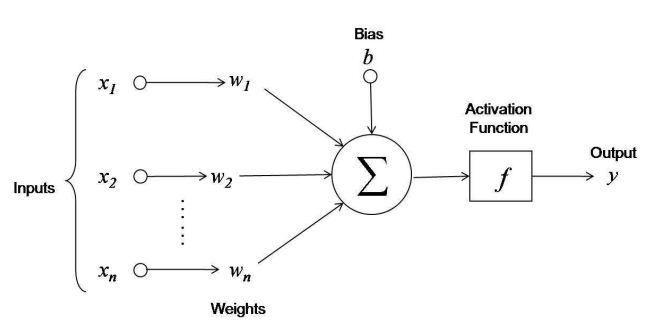
\includegraphics[scale=0.50]{image/neuron.jpg}
	\caption{A simple neuron}
	\label{neuron}
\end{figure}

\subsubsection{Neural Networks}

A neural network is a directed graph with neurons as its node. Neurons are computational units connected by directed links. Each link has its own weight that determines its importance or strength. Similarly all the computational units consist of activation functions that are applied to the input. The activation function can be any linear or non-linear function such as sigmoid $(\sigma)$, hyperbolic tangent (tanh), rectified linear units (RELU) etc. So, an output of any computational unit is a function over sum of the weighted inputs. Consider a computational units with activation function $f$ that takes inputs $x_{1},x_{2},...,x_{n}$ with weights $w_{1},w_{2},...,w_{n}$ and bias $b$ as shown in Figure \ref{neuron}. It can be  formally expressed as:


\begin{align}
z & = \sum_{i=1}^{n} wx_i + b \\
y & = f(z)
\end{align}

In this section, the working of a simple neural network is explained. A simple neural network with two inputs $a$ and $b$, one hidden unit $c$, and an output unit $d$ can be visualized as shown in Figure \ref{net}. Consider a sigmoidal function as the activation function in node $c$ and $d$. This network can be trained by optimising its weights $[W_{ac}, W_{bc}, W_{cd}]$ based on an objective function. The training has two phases : forward pass and backward pass.

\begin{figure}[h]
	\centering
	\caption{Netural Network}
	\label{net}
	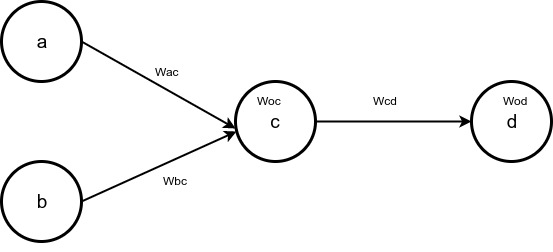
\includegraphics[scale=0.44]{image/Trace_Back_Prop.jpg}
\end{figure} 



\subsubsection*{Forward Pass}

For node c, $in_{c}$ is computed from the given weights and the input. The $in_{c}$ is fed into the activation function to get the output $A_{c}$. The output $A_{d}$ of Node $d$ is computed in the same way.
\begin{align} 
in_{c}	& = W_{ac} \times a + W_{bc} \times b + W_{oc} \\
A_{c} & = \frac{1}{1+exp(-in_{c})} \\
in_{d}	& = W_{cd} \times A_c + W_{od} \\
A_{d} & = \frac{1}{1+exp(-in_{d})} 
\end{align}

%For Node d, $in_{d}$ is computed from the given weights and the output $A_{c}$ of the previous node c. The $in_{d}$ is feed into the activation function to get the output $A_{d}$  
%\begin{align*} 
%
%\end{align*}

\subsubsection*{Backward Pass for weights adjustments}
The total loss of the networks is computed using the objective function $L = \frac{1}{2} (y - A_{d})^{2}$, where y is an actual output and $A_{d}$ is the predicted output. The gradient of loss $L$ is calculated with respect to all the weights.

For example, gradient of loss computed with respect to $W_{cd}$, 

\begin{align*} 
\frac{\partial L}{\partial W_{cd}} & = \frac{\partial L}{\partial A_{d}} \times \frac{\partial A_{d}}{\partial in_{d}} \times \frac{\partial in_{d}}{\partial W_{cd}}    \\
& = \delta_{d} \times  \frac{\partial in_{d}}{\partial W_{cd}}  \\
& = \delta_{d} \times  \frac{\partial ( W_{cd} \times A_c + W_{od})}{\partial W_{cd}}
\end{align*}
\begin{align}
& = \delta_{d} \times  A_c
\end{align}  
% the rate of change of loss (gradient) \textit{w.r.t} all the weights are calculated. 
where $\delta_{d}$ is a modification error. Weights are updated based on the gradients as shown below.
%The weight update rule in between layers i and j are 

\begin{align} 
W_{c,d} \leftarrow W_{c,d} + \alpha \times A_{c} \times \delta_{d}
\end{align}

where $\delta_{d}$ is a modification error,

%\begin{center}
%	
% gradient of Loss w.r.t $A_{d}$ $\times$ gradient of activation output $A_{d}$ w.r.t $in_{d}$.
%\end{center}

If there is more than one output unit in the layer, the partial derivative of the error across all of the output units, is equal to the sum of the partial derivatives of the error with respect to each of the output units.


%Earlier, neural models proposed used have many hidden layers as it approximates any function.



\subsubsection{Word Representation}

\cite{bengio2003neural} proposed a language model based on a neural network that predicts the next word in a sequence. They also noticed that this prediction model helped in learning a vector representation for words called word embeddings or word representations.
%The representations was learnt by starting with the random vectors and shifting its vector closer to the vector of its neighbouring words through out the training process\footnote{wrong. The vector moves close to words with similary meaning. }. 
Later in 2008, \cite{collobert2008unified} showed that these word representations can be used as an input for various downstream tasks.
%the effective use of pre-trained word vectors in various task was explained by . 
Inspired by these models, \cite{mikolov2014word2vec} proposed two novel methods: 1) Skip-Gram with Negative Sampling (SGNS); 2) Continous Bag of Words(CBOW) models for learning word representations. In the next section, we will discuss the SGNS model as it is widely adopted and used as an input for many sentence representations model \citep{kiros2015skip}.
%objective has been adapted by a sentence representation model and made a important contribution in learning generalizable sentence representations . This model was demonstratd to be inexpensive compared to previous models and performed very well in capturing the general syntactical and semantic information. The training objective of these models is to learn word vector representations that are good at predicting the surrounding words. The detailed architecture of the skip-gram model is shown in figure \ref{skipgram}. 

\begin{figure}[!tbp]
	\centering
	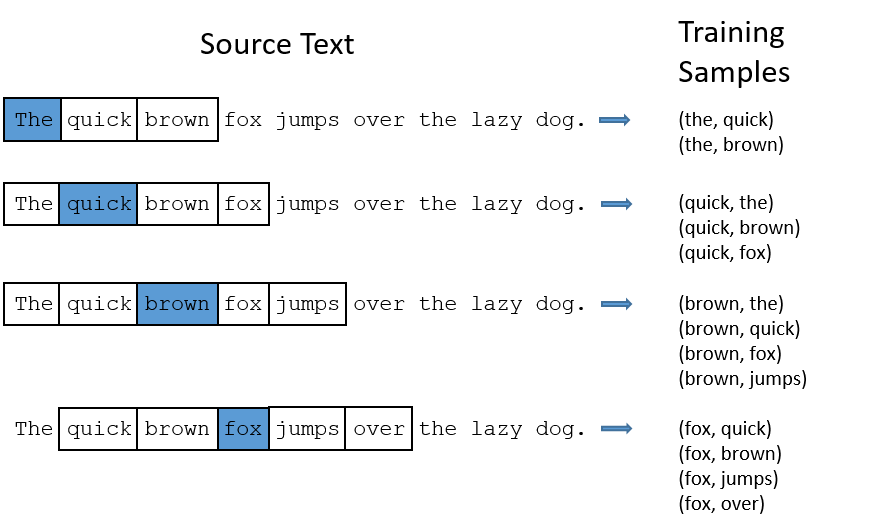
\includegraphics[scale=0.70]{image/train_samples.png}
	\caption{Training samples for skip-gram - Words pairs from raw corpus}
	\label{train_sam}
\end{figure}

%The primary goal of skip-gram model is to learn the weights of the hidden layer which transforms to the word vector representation undergoing the process of training.\footnote{The goal of skip gram was just to predict word based on context. You just said this in last sentence.} Given any word in the vocabulary $V$ from a training corpus, skip-gram model outputs probability that determines how likely the words in the vocabulary can appear near to the source word.\footnote{Third time same concept in different words} 


The SGNS model is trained on a monolingual text corpus, where every center word is used to predict the surrounding words within a window size as shown  in Figure \ref{train_sam}.
%using samples consisting of word pairs derived from raw text corpus with a defined window size as shown in Figure.
The model takes word input in the form of One-Hot vector of dimension $1\times|V|$. While building a vocabulary from the training corpus, One-Hot vector $1\times|V|$ is assigned to each word consisting of value 1 in the position that is the same as the position of the word in the vocabulary, and value 0 in all other positions. This input vector X is multiplied with the word matrix $W$, to get the hidden layer $v$ (target word representation) of dimension $1\times|D|$, where D is the dimension of word representation. To find the context word score, the dot product is performed between the hidden layer and the context matrix as shown in Figure \ref{C_W_matrics}. For each word, the context word score is normalised using softmax function, to get the probability of each word in the vocabulary occurring near the given word. 



For a word $w_{j}$, the probability of any $k^{th}$ word in V is calculated by

\begin{align}
p(w_{k} | w_{j}) = y_{k} = \frac{\exp( c_{k} \cdot v_{j})}{\sum_{i=1}^{|v|} \exp(c_{i} \cdot v_{j}) }
\end{align}

\begin{figure}[!tbp]
	\centering
	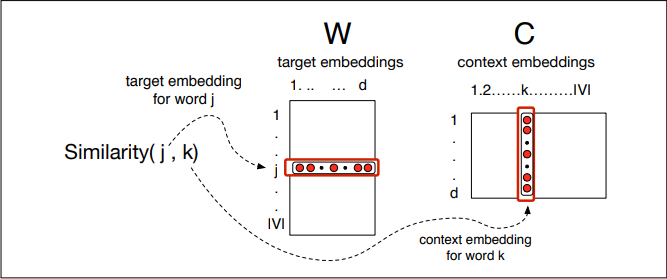
\includegraphics[scale=0.50]{image/cbows.png}
	\caption{Context and Word matrices \citep{jurafsky2014speech}}
	\label{C_W_matrics}
\end{figure}

The output of the network is the vector $1\times|V|$ consisting of the probability distribution of each word in the whole vocabulary. Each probability value in the vector position denotes the likelihood of a word corresponding to the same position in the vocabulary. The weight parameters in this network are tuned by using cost function $L$

\begin{align}
L = - \log ( p(w_{O,1}, wO,2, . . . , w0,C|wI))
\end{align} 

The prediction error is calculated by taking the derivative of $L$ with respect to input units of output layer and hidden layer. The learning algorithm is started with the randomised word and context matrices (weight parameters of this network). Optimiser algorithms such as Stochastic Gradient Descent are used to tune the weight parameters using error backpropagation to broadcast the gradient through the network. Later, the Skip-Gram model was improved by replacing the Softmax function in the output layer with Negative Sampling. This model provided state of the art performance while testing for semantic and syntactic word similarities. \citep{mikolov2014word2vec}. 


\begin{figure}[!tbp]
	\centering
	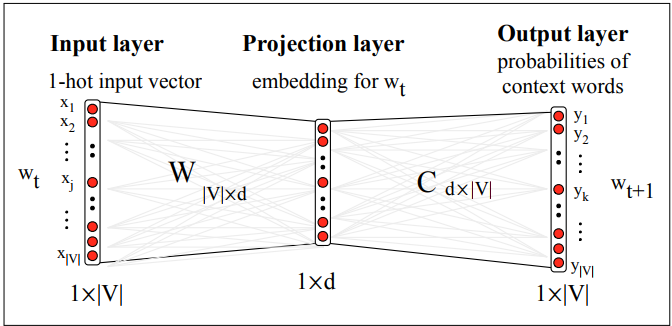
\includegraphics[scale=0.50]{image/skip-gram.png}
	\caption{Skip-gram Model \citep{jurafsky2014speech}}
	\label{skipgram}
\end{figure}

\subsubsection{Sentence Representation Model}
As word representation models became very useful and predominantly used, a natural next step was to extend such approaches to sentences. The goal was to learn a general sentence representations that would capture its semantics using previously trained word representation.
%As the models proposed for learning word representations are well established models and proved to be successful in their performance, recent research has focused models that can learn a general sentence representations that would capture its proper semantics using previously trained word representations. 
The vector representations can be learned by using two approaches 1) Supervised models \citep{conneau2017supervised} 2) Unsupervised models \citep{kiros2015skip}. Skip-gram model is unsupervised learning as its objective function was to optimise the word representations. In this type of learning, general information is captured. The knowledge captured by these models can be transferred to any NLP task that needs to process a sequence. Supervised learning of vector representations is training a model on a pre-defined task, with defined input-output samples where the model parameters are optimised based on the task. The word representations are learned in internal states as the model is trained on an STS task. In this type of learning, the model learns the information that is specific to the task and fails to capture general knowledge. All proposed models aim to generate an efficient sentence representation that consists of the whole meaning with context. This is important as it can be used for various tasks with minimal adaptation. This property results in smooth transfer of learning to the model that learns any specific task. By promoting Transfer Learning, the training complexity and training time for specific tasks decreases.  

\subsubsection{STS Features and Accurracy}

For STS task, traditional machine learning algorithms used handcrafted features from the raw sentence such as word overlap, knowledge based similarity, length features and other similarities. Neural models use word representation to train the models. Recently neural models \cite{conneau2017supervised} \citealp{kiros2015skip} \cite{shao2017hcti} have been popular as they outperform all the traditional machine learning algorithms. Ensemble techniques which combine the prediction techniques of traditional machine learning models and neural models are also being explored.


The performance of the model is measured using Pearson Correlation of the predicted score with a human judgment score given in the dataset \citep{agirre2015semeval}. Generally, correlations measure the extent to which two variables change together. Pearson Correlation, meaures the direction of linear relationship between pairs of continous variables that are well suited for the sentence relatedness task.

\subsubsection{STS Dataset}

For training and testing of the STS model, I use data published in SemEval 2012-SemEval 2017. It includes the collection of STS dataset created using corpus from various domains. The training data domains include 1) news headlines from the RSS feed of the European Media Monitor; 2) image captions from Flickr; 3) pairs of answers collected from Stack Exchange; 4) student answers paired with correct reference answers from the BEETLE corpus; 5) forum discussions about beliefs from the DEFT Committed Belief Annotation dataset \citep{agirre2015semeval}. 


\chapter{Related Work}


Despite developing a number of learning algorithms for representing words and sentences, generating high quality and efficient sentence representations remains an unsolved problem \citep{conneau2017supervised}. An efficient sentence representation that consists of the whole meaning with context is important as it can be used across various tasks with minimal adaptation. This property results in a smooth transfer of the learning to train any NLP task. We focus on the STS task, as \cite{conneau2017supervised} demonstrated that natural language inference tasks appear to capture more generalisable sentence representaion using Transfer learning. This project proposes to compare and study different models used for STS tasks to infer how they impact in learning good sentence representations.

\subsection{Traditional Machine Learning Models}

For decades, traditional machine learning algorithms such as support vector machine or logistic regression were to used to solve any NLP tasks. In 2012, supervised models based on the lexical and syntactic features of the sentence pair showed promising results on measuring semantic relatedness. These systems gave 52\% - 59\% correlation on various datasets by using regression models consisting of various similarity measures as its input features. The unsupervised models did well for next two years in row using the WordNet knowledge and the LSA similarity measures which assume that the words with closer meaning highly co-occur in the text corpora. 

\cite{han2013umbc_ebiquity} proposed three approaches that involved 1) LSA similarity model, 2) semantic similarity model based on the alignments quality of the sentences, and 3) support vector regression model that had features from different combinations of similarity measures and the measures, from two other core models. It was observed that using n-gram overlap feature increased LSA similarity model. Out of three models proposed by \cite{han2013umbc_ebiquity}, the alignment based system gave 59\% - 74.6\% pearson correlation on four different datasets. Using this model's alignment quality as one of the features in the Support Vector Regression model improved the correlation score to 78 \%.  Various supervised models using unigram (one word) or bigram (two words) overlap, vector distance, and cosine similarity of sentence embedding, were proposed \citep{agirre2015semeval}.   

\cite{tian2017ecnu} proposed a system that adapted ensemble learning techiques to solve the Textual Entailment and STS tasks, using the same set of features. The combination of classical NLP models like Support Vector Machine, Random Forest, Gradient Boost and a deep learning model are used in this system. For classical NLP models, single sentence and sentence pairs feature sets, are hand engineered based on properties like N-gram overlap, syntax, alignments, word sequence, word dependency, word representations etc.. In SEM-EVAL 2017, this mixed ensemble model gave 81 \% Pearson Correlation outperforming all the neural models presented in that shared-task event.

Although using hand-crafted features in the above mentioned models works, it has some drawbacks such as tuning the features extracted on addressing the corpus from new domains, high computational complexity in hand engineering the features, effective feature selection etc.. Recent approaches in deep learning continue to prove that the problem of semantic text matching can be handled in an efficient way \citep{cer2017semeval}. The problem of semantic word matching can be extended to solve the problem of the semantic sentence match by using deep learning approaches. This helps when it comes to effectively learning the word meanings in the sentence individually and deriving a meaningful sentence representation from the word vectors.  

\subsection{Neural Models} 

This section discusses the top ranking neural models presented in Sem-Eval 2017 that have been proposed to build sentence representations and predict sentence relatedness.

\cite{kiros2015skip} proposed the Skip-Thought model based on skip-gram objective from \cite{mikolov2014word2vec}. For any three consecutive sentences in the document $S_{i-1}, S_{i}, S_{i+1}$, the Skip-Thought model predicts the previous sentence $S_{i-1}$, and next sentence $S_{i+1}$ given any sentence $S_{i}$.
This work focuses on training an encoder-decoder model. A variant of recurrent networks consisting of gated recurrent units (GRU) \citep{cho2014learning} is used as an encoder to map input sentences into a generic sentence representation. RNN with conditioned GRU is used as a language model to decode the sentence representation and predict surrounding sentences $S_{i-1}$ and $S_{i+1}$. In evaluating a semantic relatedness task, Skip-Thought outperformed all systems proposed in a shared task SemEval 2014 \citep{marelli2014semeval}.
%and was outperformed by dependency Tree-LSTM model.

\cite{tai2015improved} proposed a recurrent neural networks(RNN) with tree based LSTM units with two variants Child-Sum Tree-LSTM and N-ary Tree LSTM. Given a sentence syntactic structure in form dependency tree of the words, Tree-LSTM networks are capable of integrating the child node's information. The Tree-LSTM units in each node t consist of input gate $i_{t}$, output gate $o_{t}$, a cell unit $c_{t}$ and a hidden output $h_{t}$. Unlike Standard LSTM, the parent node has one forget gate $f_{tk}$ for each child node \textit{k} in the Tree-LSTM. This property allows selective usage of child information. Previously proposed RNN models with sequential LSTM units, have limited ability to capture the meaning difference in the two sentences raised due to word order and synactical structures. Tree-LSTM addresses this issue by computing its hidden layer output as a function of the outputs from its children hidden units and input vector. 

In modelling semantic relatedness, the input $x_{t}$ denotes the word vectors of the sentence parse tree. The proposed model retains the information of more distant words from the current words compared to other exisiting models. These properties make the model effective in highlighting the semantic heads in the sentence. It also captures the relatedness of two phrases which have no word overlap. With these properties, Tree LSTM performs better than existing sequential RNN-LSTM models, and models with hand engineered features on predicting the semantic relatedness of two sentences. But one major downside is that the dependency tree-LSTM relies on parsers for dependecy tree input, which is computationally expensive to collect and does not exist for all languages making it inefficient in cross-lingual sentence representations.



\cite{shao2017hcti} presented a simple Convolutional neural network model for STS tasks. This model constsis of CNN model and fully connected neural network (FCNN). CNN takes pre-trained word vectors from Glove \cite{pennington2014glove} enhanced with handcrafted features as its input. It enhances word vector to task specific forms in the convolutional layer and max-pooling generates the task-dependent sentence representation. FCNN generates the similarity score ranging from 0-5. This model ranked 3rd in SemEval-2017 with 78 \% correlation on STS task. 


\cite{pagliardini2017unsupervised} proposed a simple unsupervised objective Sent2Vec, to train a generic distributed representation for sentences. The main contribution of Sent2Vec is its low computational cost for both training and inference relative to other existing state-of-art model. This model is an extension of CBOW training objective from Word2Vec \citep{mikolov2014word2vec}, to sentence context.


\cite{conneau2017supervised} investigated the performance of various supervised encoders in learning universal sentence representations. They hypothesized that textual entailment task is a good choice for learning universal representations and demonstrated the hypothesis with various enoder models. To prove that the sentence representations learned are universal, the representations learned from unsupervised and proposed hypothesis was used in 12 different transfer tasks such as Caption-Image retrievel, Paraphrase detection, Entailment/semantic relatedness, sentiment analysis etc.. As the result of their experiments, Bi-LSTM with max-pooling trained on Natural Language Inference Task (Textual Entailment), generated the best sentence representations, and outperformed SkipThought \cite{kiros2015skip} and FastSent \cite{hill2016learning}.

\chapter{Proposed Work}

A wide variety of supervised and unsupervised encoders for learning sentence representation have been proposed by NLP researchers in recent times. However, there is a lack of understanding about the characteristics of different encoding techniques that can capture useful, generic semantic information \citep{conneau2017supervised}. Supervised neural models suffer from an inherent bias toward the task and dataset that they are trained on.
%captures the bias in the dataset effectively. 
This feature is a downside because it learns the task very well and fails to capture generic useful information during the training time, leading to poor generalization. On the contrary, unsupervised learning models give more importance to general information, therefore, failing to specialize the model for any specific task. 

Many factors affect how the basic semantics of a sentence are being captured during training. An important factor to note is the task in which the model is trained. Similarly, the encoders' architecture for both supervised and unsupervised neural models also impacts learning in different ways. A comparison study on these encoder's architecture will enable us to gain insight on its efficiency in capturing better sentence representations.

%To infer more insights on the techinques that yield state of the art performance on capturing the semantics of the sentence, we compare few models presented in SemEval-2017 \cite{cer2017semeval} that showed promising results on STS shared task.

In this project, I propose to perform  a systematic comparsion of different encoder techniques for generating sentence representations and their ability to capture semantics of the sentence. To do this, I am implementing and studying the following models: support vector machine (SVM), Random Forest (RF), Convolutional Neural Network Encoder \citep{shao2017hcti} and BiLSTM RNN with max-pooling \citep{conneau2017supervised}. The models proposed in \cite{shao2017hcti} and \cite{conneau2017supervised} are the best performing models in STS tasks. These models will be implemented using sci-kit learn, PyTorch and Keras library. \cite{conneau2017supervised} demonstrated that Recognizing Textual Entailment (RTE) captures semantics very well. Based on this inference, we will train the  encoders on Standford Natural Language Inference (SNLI) corpus  \citep{bowman2015large}, and Sentences Involving Compositional
Knowledge (SICK) dataset \citep{marelli2014semeval}, for semantic relatedness and RTE tasks.

The main objective of this comparison study is to understand the efficiency of the sentence representations models and to answer the following questions:

\begin{itemize}
	\item What are the vital features in prediction while using machine learning models ?
	\item How do we measure effectiveness of the traditional machine learning models ?
	\item What are the trade-offs incurred by neural networks as opposed to the traditional machine leanrning models?
	\item What is the impact of various activation functions used in the encoders hidden layers?
	\item What is the preferable neural network architecture for learning better sentence representations? 
	\item What are the impact of various optimisers in training a model?
	\item Since the dimensionality has direct effect on the memory requirements and processing time, what dimensionality size has good trade-off between accuracy and training time? 
\end{itemize}
 
\chapter{Evaluation}
In this project, the performance of the models proposed for STS task is evaluated using two metrics, 1) Accuracy of its prediction; 2) Training Time. The accuracy of the STS models is measured using Pearson correlation between machine generated semantic score and gold standards created using human judgement. It helps in capturing the linear relationship between the predicted and target semantic score. This correlation value ranges from -1 to 1 where, 1 indicates perfect positive correlation and -1,0 indicates no or negative correlation. 
 
 Although complex models give better accuracy, they take a long time to train. Analysing the training time of the encoder models help in finding a tradeoff between the training time and the model performance. To perform this analysis, all the models implemented in this project will be trained using a machine with 4 $\times$ CPUs, 16GB RAM and 1 $\times$ NVIDIA Tesla K80 GPU.  

The evaluation metrics discussed in this section will be used for the comparison study. In addition, the sentence representations encoders are evaluated for its performance on generating a generic sentence representation that aids in transfer learning. This evaluation is carried out by using representations learned from training RTE task as input in sentence relatedness task and vice versa. Generic representations are expected to perform well in both tasks in terms of accuracy.
	   
%Both the RNN models investigated with mean and max pooling over the hidden representations separately. 

	 
%	 , far less is known about  across many task. for representing the sentence that captures semantics and syntactic  focusing on the semantic relatedness and diferent appro

\section{Implementations}
%	\subsection{Feature Engineering}
I have implemented the models proposed in \cite{shao2017hcti} and measured their performance using Pearson's Correlation. In this section, the implementation details of one of the model architectures used for the comparison study are discussed. Two other models are yet to be implemented.
	
	\subsection{A Simple CNN Model For STS Task}
		This section explains the convolution neural networks(CNN) based learning model used for semantic sentence similarity. The two main components of this model are (CNN) based sentence representation model, and fully connected neural networks (FCNN) used as the multi-class classifier. The CNN architecture consists of two convolution networks that work parallel to mapping the two sentences to a vector space. The distributional vectors of the sentence pairs are used by FCNN to classify their sentence similarity score. In the following, we first describe our sentence model for mapping sentence pairs to their intermediate representations and then explain how these representations are used to classify the relatedness score.
	
	\subsubsection*{Sentence Model using CNN}
	Our CNN architecture for mapping sentences to feature
	vectors inspired from \cite{shao2017hcti} is shown in Figure 1. This architecture consists of two 1-dimensional convolution layers and a max pooling layer. The objective of this network is to convert the raw sentence into vector representations from \cite{pennington2014glove}, using pre-trained 300 dimension word embeddings of all the words \{$w_{1}, w_{2},...,w_{|s|}$\} present in the sentence.
	
	The input sentence to the convolution layers is treated as a sequence of a real valued number where the real valued integers are retrieved from the integer-word mapping present in the vocabulary V. The vector representaion of all the words $ w \in \mathbb{R}^{d}  $ are drawn from embedding matrix  $ W \in \mathbb{R}^{d \times |V|} $ in the embedding layer. To enhance the word representation with respect to this task, a true flag for word overlap is added as an additional dimension into the word vector representation for each word in the sentence. Then the CNN network applies the convolution and max pooling operation to find the optimal feature vectos for the sentence that capture its semantics. 
	
	The idea behind the convolution layer is to learn the features which identified the relationship between n-gram of the sentence using weight vectors \textit{m} $\in \mathbb{R}^{|m|}$ . The $1 \times 1$ weight vector \textit{m} also known as filters of the convolution is used. This convolution operation is followed by applying Relu activation function to learn non-linear decision boundaries. This filters out the insignificant features learned in previous operation. The output from the convolution layer is passed to the max pooling layer with pool size (1, $|S|$) where the semantic information learned is aggregated, and reduuces representation dimension from $1 \times |S| \times 300$ (word vec dimension) to $1 \times 300$ (word vec dimension).The convolution layers along with RELU activation function and max pooling acts as a non linear  feature detector for the given sentence. The output sentence representation from CNN is used to find the Semantic Difference Matrix by performing a series of operations on the two sentence vector. 
	
	\begin{figure}[!tbp]
		\centering
		\begin{minipage}[b]{0.43\textwidth}
		\centering
		\label{CNN_1}
		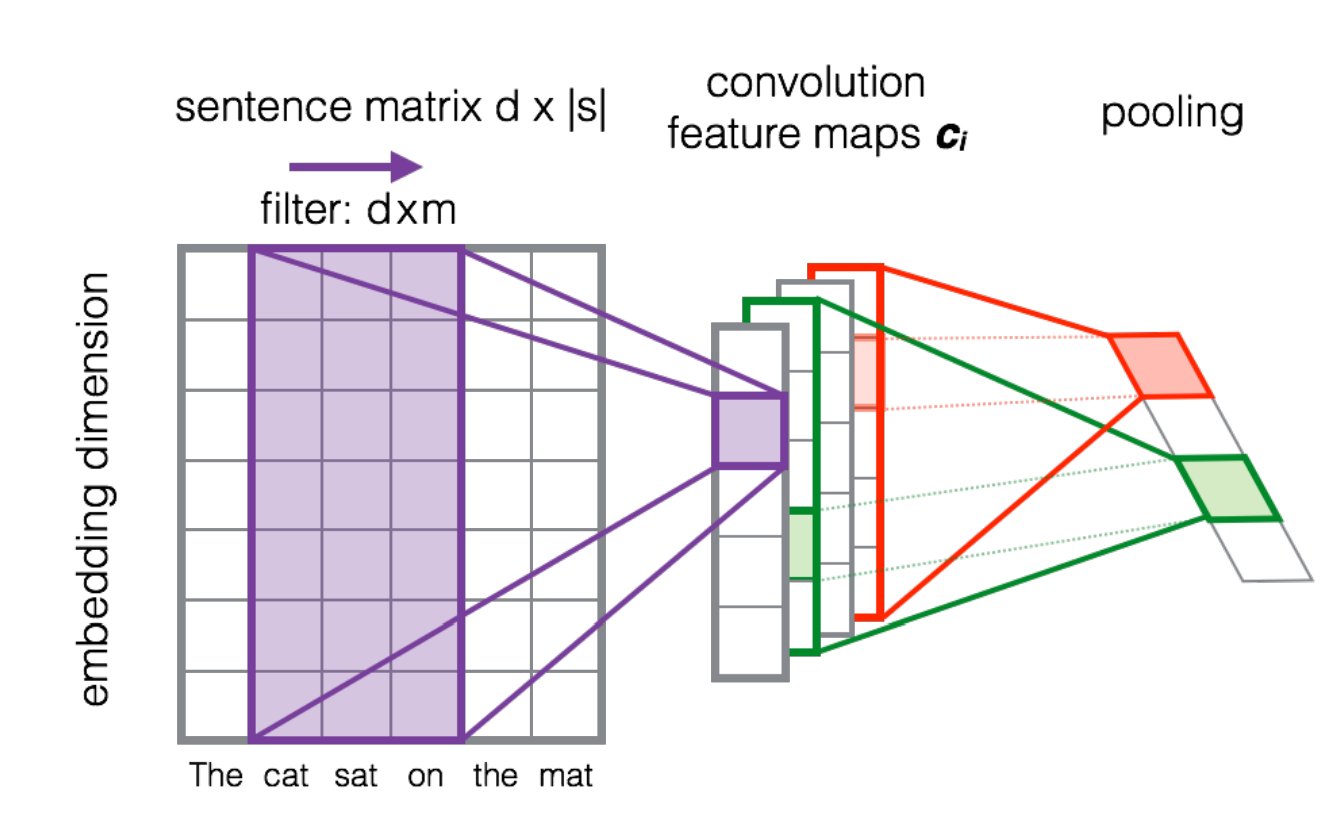
\includegraphics[scale=0.20]{image/CNN_sentModel.png}
		\caption{CNN Sentence Model \cite{severyn2015learning}}
		\end{minipage}
		\hfill
		\begin{minipage}[b]{0.3\textwidth}
		\centering
		\caption{Hyperparameters for FCNN \cite{shao2017hcti}}
		\label{params}
		
		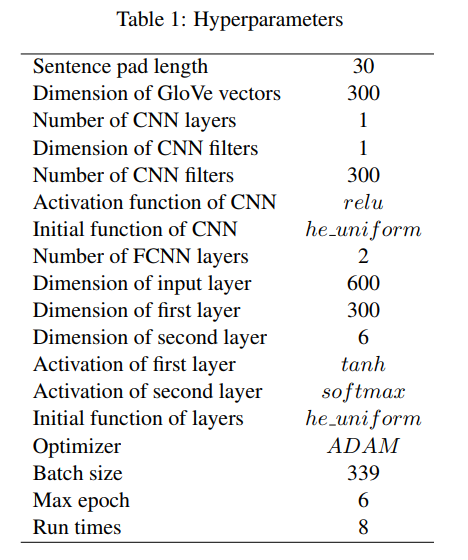
\includegraphics[scale=0.35]{image/hyperparameters.png}
		
		\end{minipage}
	\end{figure}
	
	
	\subsubsection*{Semantic Difference Matrix}
	The semantic difference matrix is generated by concatenating the vector difference and vector product of a two sentence representation. This matrix is used to classify the similarity measure using fully connected neural network (FCNN) with 2 dense layers. 
	
		\begin{align*} 
			SDV & =(|SV_{1}- SV_{2}|.(SV_{1} \circ SV_{2})) \\
		\end{align*}
	
	\subsubsection*{Similarity Measure using FCNN}
	
	 This network consists of one hidden layer a 300 node size, and an output layer of a size 6. The hidden layer applies a \textit{tanh} activation function and the output layer applies softmax layer. The softmax layer calculates the probability over the six score labels. The hyper parameters of this network is shown in Figure \ref{params}.
	 
	 Finally, the model is trained using the categorical cross-entropy loss: given a vector of probabilities p for a training pair of sentences, if the correct similarity category corresponds to index i of p, the model will evaluate the loss as $L = − log(pi)$.
	 	
	\section{TimeLine}
	In this section, the timeline regarding my project is discussed. I have completed implementing the CNN model with a small dataset and reproduced the results stated in \cite{shao2017hcti}. For ensemble models and traditional models, I have implemented a model to hand engineer 71 features categorised under single sentence features and sentence pairs features. This model and InferSent will be further discussed in future reports. 
	
	\begin{table}[ht]
		\centering
		\caption{TimeLine}
		\label{my-label}
		\begin{tabular}{|l|l|l|}
			\hline
			Task                          & Task Period &             \\
			\hline
			Literature Survey             & Nov - Jan   & Completed   \\
			\hline
			Implementation - Traditional ML models & Dec         & Completed   \\
			\hline
			Implementation - CNN Model   & Nov         & Completed   \\
			\hline
			Implementation - InferSent   & Jan - Feb   &  InProgress \\
			\hline
			Proposal                      & Jan 18        & Under review          \\
			\hline
			Project Report                & Jan - Mar   & In-Progress           \\
			\hline
			Project Defence               &       -      & - \\    
			\hline       
		\end{tabular}
	\end{table}
   
\bibliographystyle{plainnat}
\bibliography{sample}   

\end{document}